\chapter{Vorgehen}
\label{chap:vorgehen}

% Dieses Kapitel beschreibt das methodische Vorgehen, welches in der Arbeit angewendet wurde. Erwähnen Sie hier die verschiedenen Phasen der Arbeit und ihre Ergebnisse. Arbeiten mit hohem Softwareentwicklungs-Anteil lehnen sich am besten an eine etablierte Vorgehensweise an wie zum Beispiel Scrum, XP oder Agiler UP. Detailierte Projektpläne, Deliverables und anderes, falls vorhanden, gehören aber in den Anhang.
\section{Projektphasen}
\label{sec:projektphasen}

Um bei der Arbeit strukturiert vorzugehen, wurden folgende Projektphasen gewählt:
\begin{itemize}
\item Erarbeitung und Festhaltung der Anforderungen
\item Erarbeitung der formalen und technischen Grundlagen
\item Modellierung der Ontologie
\item Erstellung der Dokumentation zur Wissensmodellierung
\item Erarbeitung der praktischen Grundlagen
\item Erstellung der abschliessenden Dokumentation
\end{itemize}

Dabei ist zu sagen, dass die Phasen der Modellierung der Ontologie sowie der Erstellung der Dokumentation zur Wissensmodellierung grösstenteils parallel abliefen bzw. Hand in Hand übergingen. Die während der Modellierung erhaltenen Erkenntnisse konnten direkt in die Dokumentation übernommen werden.

\subsection{Anforderungen}
\label{subsec:anforderungen}
In der Projektphase der Anforderungen wurden die Anforderungen an die Arbeit erarbeitet. Ergebniss dieser Phase ist ein Anforderungsdokument mit den wichtigsten Eckpunkten, siehe~\autoref{sec:anhang:anforderungen}. Es wurde ursprünglich festgehalten, dass der praktische Teil der Arbeit --- die Erarbeitung einer Ontologie anhand einer Wissensdomäne --- mittels eines konkreten Anwendungsproblems, der Erlernung der Programmiersprache Prolog, umgesetzt werden soll. 

Im Laufe der Arbeit hat sich jedoch gezeigt, dass semantische Netze bzw. Ontologien nicht ein geeignetes Mittel sind um Logiksprachen wie z.B. Prolog abzubilden. Dies wird Kapitel~\autoref{sub:modellierung_der_ontologie} genauer beschrieben.

\subsection{Formale und technische Grundlagen}
\label{sub:formale_und_technische_grundlagen}

\subsection{Modellierung der Ontologie}
\label{sub:modellierung_der_ontologie}
Ursprünglich wurde versucht ein Modell der (Logik-) Programmiersprache Prolog zu erstellen. Zuerst geschah dies mittels dem klassischen Ansatz der Modellierung mittels der Modellierungssprache UML, da die Autoren über einen Hintergrund der objektorientierten Programmiersprachen verfügen. Es wurde jeodch schnell klar, dass es nicht ausreicht nur Klassen zu definieren, da eine Ontologie nur Beziehungen zwischen Individuen abbilden kann. Daher muss sie immer über Instanzen bzw. Individuen verfügen.

\begin{figure}[H]
\centering \rotatebox{0}{\scalebox{0.3}[0.3]{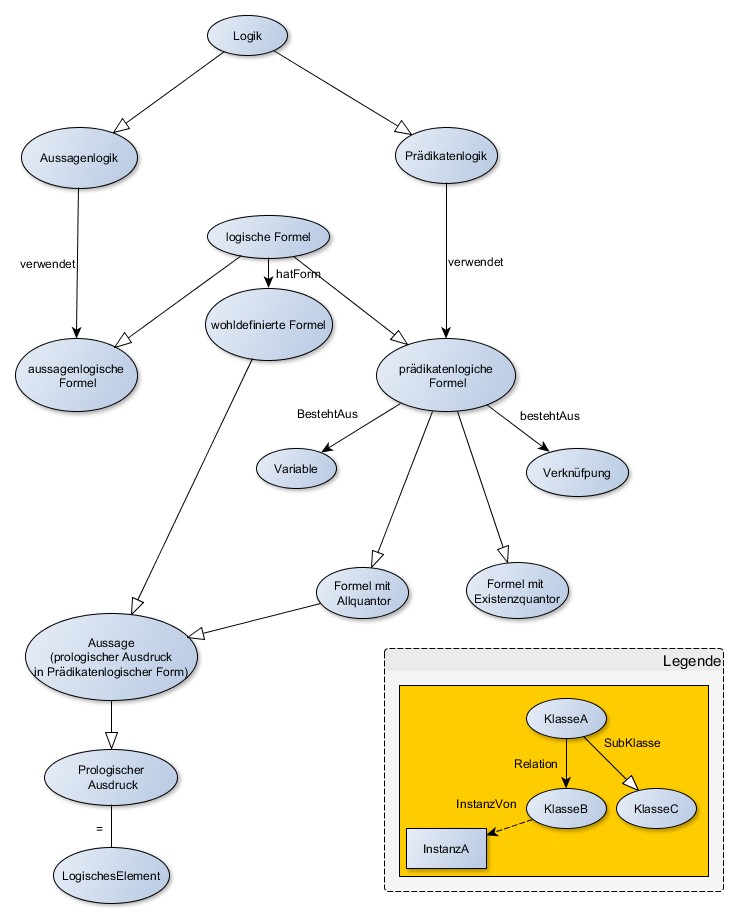
\includegraphics{bilder/formel_baum.png}}}
\caption{Vereinfachte Darstellung von Logik, rein mittels Klassen.\label{fig:prolog_logik_baum}\protect\footnotemark}
\end{figure}
\footnotetext{Eigene Darstellung mittels yEd.}

Um auch Relationen abbilden zu können wurde die Modellierung schliesslich mit Individuen erweitert. Dies erlaubte die Definition von Relationen zwischen diesen, was sich als Schritt in die richtige Richtung erweisen sollte.

\begin{figure}[H]
\centering \rotatebox{0}{\scalebox{0.3}[0.3]{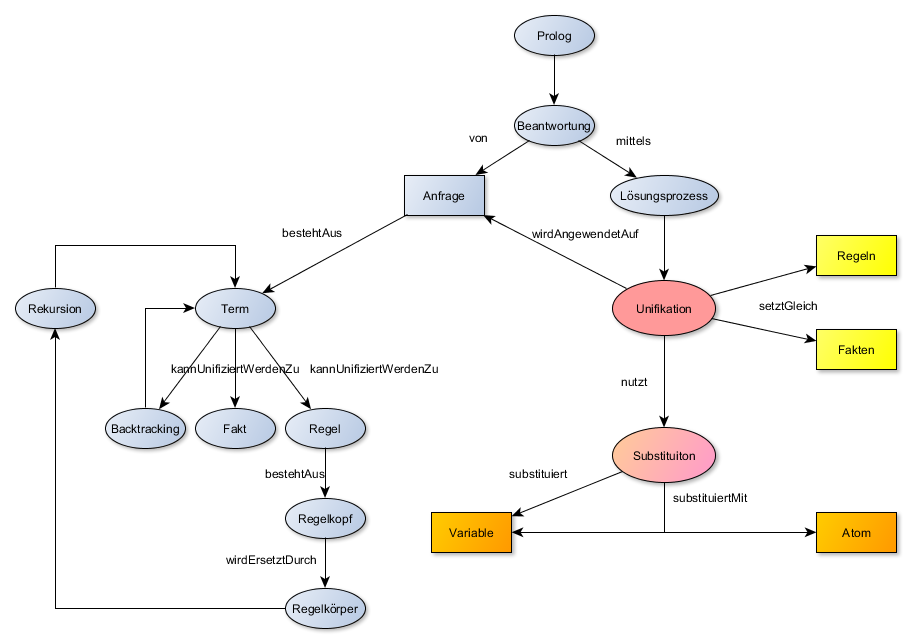
\includegraphics{bilder/loesungsprozess_baum.png}}}
\caption{Vereinfachte Darstellung eines Teils des Lösungsprozesses von Prolog, mittels Klassen, Individuen und Relation.\label{fig:prolog_loesungsprozess}\protect\footnotemark}
\end{figure}
\footnotetext{Eigene Darstellung mittels yEd.}

Es wurde dann jeweils versucht konkrete Fragen aufgrund der erstellten Ontologie zu beantworten, wodurch Mängel in der Ontologie relativ gut sichtbar wurden. Dies konnten dann schrittweise korrigiert werden, so dass die gewünschten Abfragen doch umgesetzt werden konnten. Details zu den gemachten Abfragen finden sich unter~\autoref{sec:anhang:sparql_beispiele}.

\begin{figure}[H]
\centering \rotatebox{0}{\scalebox{0.6}[0.6]{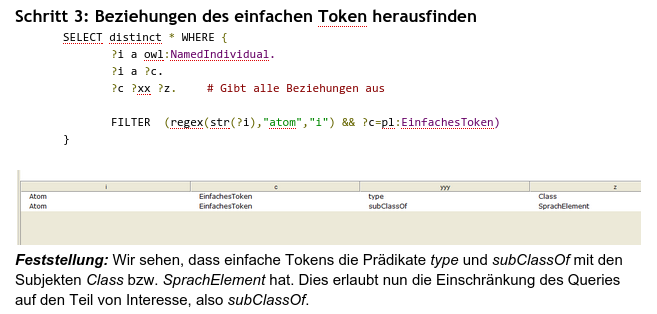
\includegraphics{bilder/sparql_beispiel.png}}}
\caption{Beispiel einer Abfrage der Ontologie mittels SPARQL.\label{fig:sparql_beispiel}\protect\footnotemark}
\end{figure}
\footnotetext{Eigene Darstellung mittels Stanford Protégé und Google Docs.}

Schnell wurde klar, dass solch eine Modellierung ins Uferlose gehen kann, woraufhin der Betreuer der Arbeit, Herr Dr.\ Eckerle, empfahl Literatur über Prolog als Grundlage bzw.\ Rahmen zu verwenden. Hierbei wurde auf das Buch \textit{Künstliche Intelligenz} von \textit{U. Lämmel} und \textit{J. Cleeve} zurückgegriffen~\cite{laemmel}. Daraus resultierte eine verbesserte Modellierung der Ontologie von Prolog, mit Klassen, Relationen und Individuen.

\begin{figure}[H]
\centering \rotatebox{0}{\scalebox{0.15}[0.15]{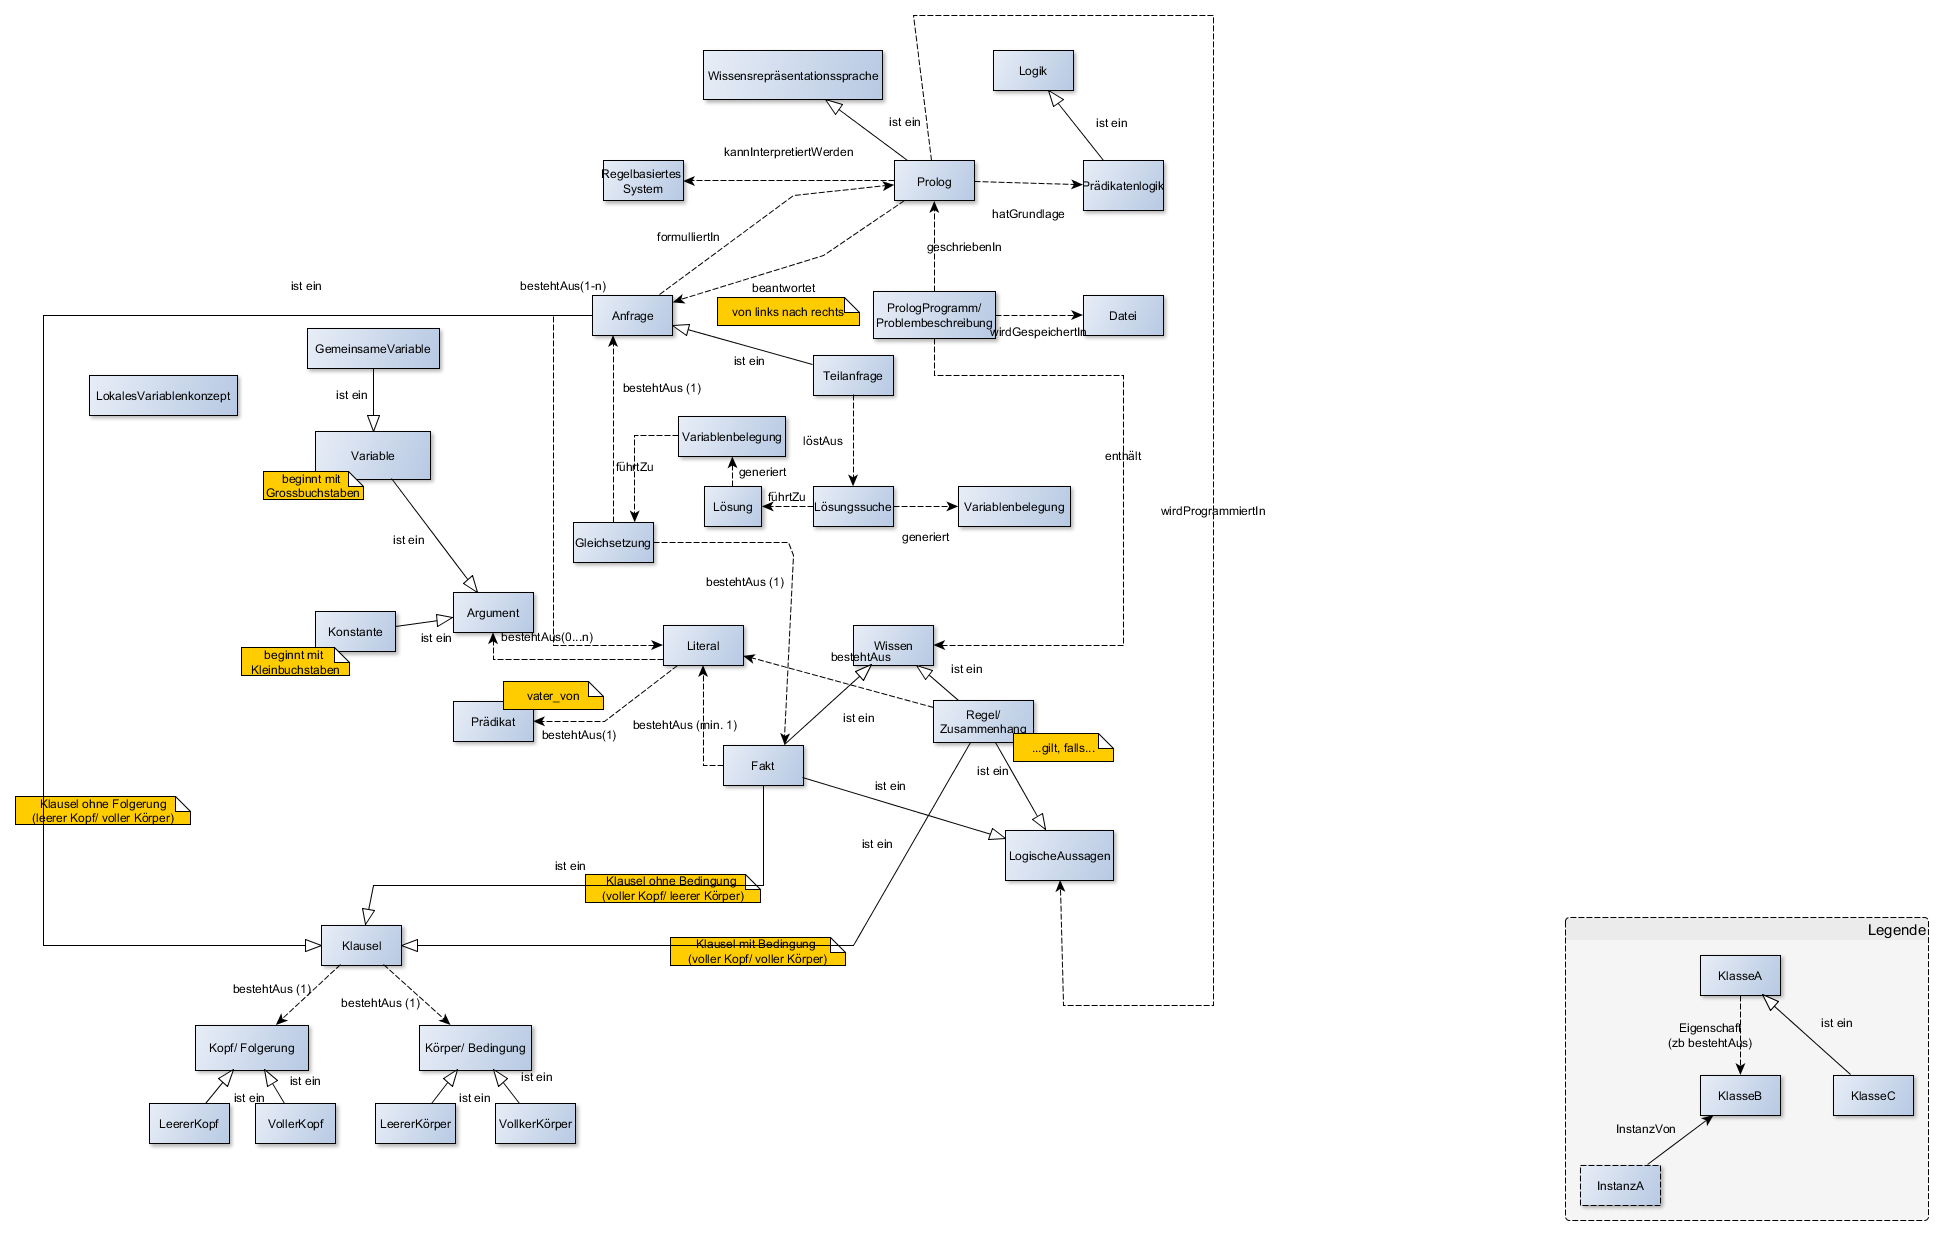
\includegraphics{bilder/prolog_baum.png}}}
\caption{Vereinfachte Darstellung von Prolog, mit Klassen und Relationen (Individuen wurden der Übersicht halber bewusst weggelassen).\label{fig:prolog_baum}\protect\footnotemark}
\end{figure}
\footnotetext{Eigene Darstellung mittels yEd.}

Dies erlaubte jedoch nach wie vor keinen zusätzlichen Gewinn von Mehrwert in Form von Inferenz. Nach diversen Gesprächen mit dem Betreuer der Arbeit, Herrn Dr.\ Eckerle, stellte sich heraus, dass der Ontologie Regeln fehlen. Es wurde dann versucht mithilfe von Prolog das Konzept von Prolog abzubilden, da dort ein Auskommen ohne Regeln nicht möglich ist bzw.\ ansonsten keine Abfragen gestellt werden können. Nach diversen, erfolglosen Versuchen Regeln zu finden, wurde dies zuerst anhand einfacher Modelle versucht, was schlussendlich auch gelang.

\begin{figure}[H]
\centering \rotatebox{0}{\scalebox{0.15}[0.15]{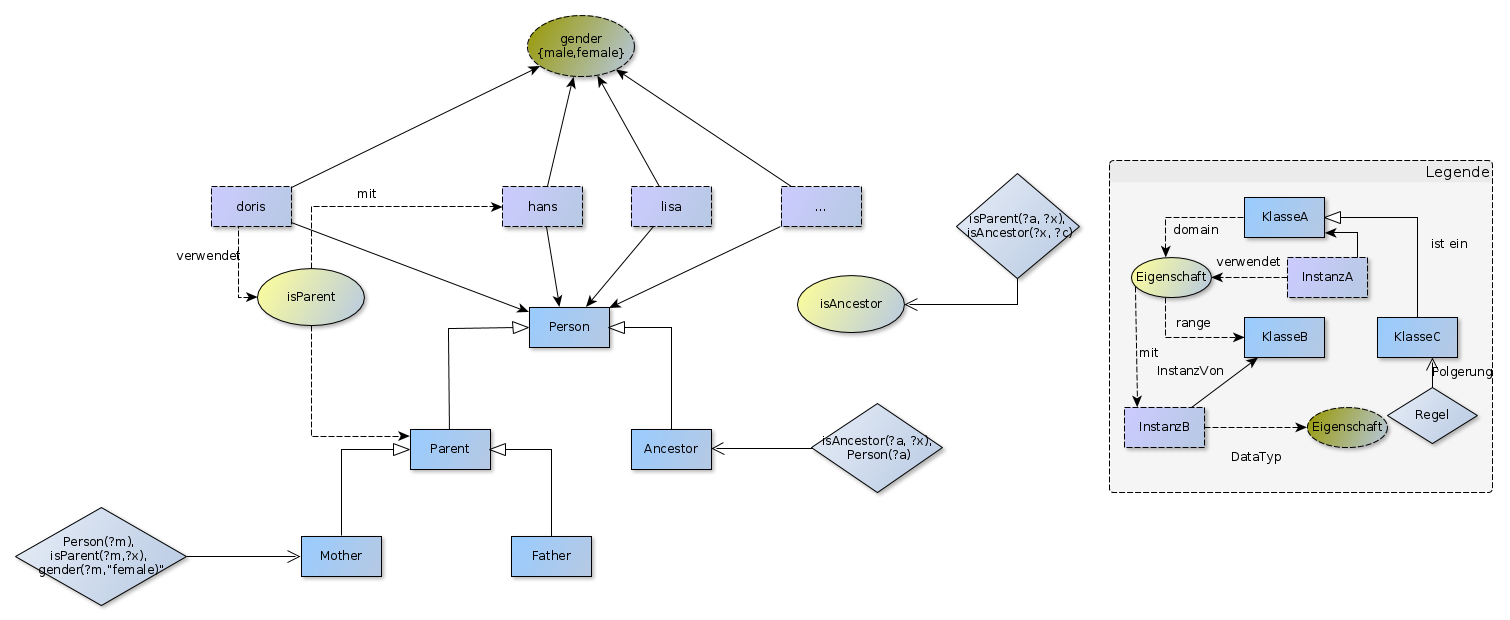
\includegraphics{bilder/familien_netz.png}}}
\caption{Darstellung eines einfachen Beispiels, der Abbildung einer Familie, mit Klassen, Individuen, Relationen und Regeln.\label{fig:familien_netz}\protect\footnotemark}
\end{figure}
\footnotetext{Eigene Darstellung mittels yEd.}

Jedoch gelang es auch nach Abbildung von Regeln anhand einfacher Beispiele nicht, Regeln für die eigentliche Wissensdomäne zu finden. Die Erkenntnis aus diesem Prozess ist schlussendlich, dass die Abbildung von Prolog in einer Ontolgie zwar möglich ist, jedoch eher in lexikalischer Form, was den Vorteil der Inferenz zunichtemacht. So kann beispielsweise gesagt werden, dass Prolog Unfikikation auf Anfragen anwendet und dabei Regeln mit Fakten gleichsetzt. Dabei wird Substitution genutzt, welche Variablen mit Variablen und/oder Atomen substituiert.

\begin{figure}[H]
\centering \rotatebox{0}{\scalebox{0.2}[0.2]{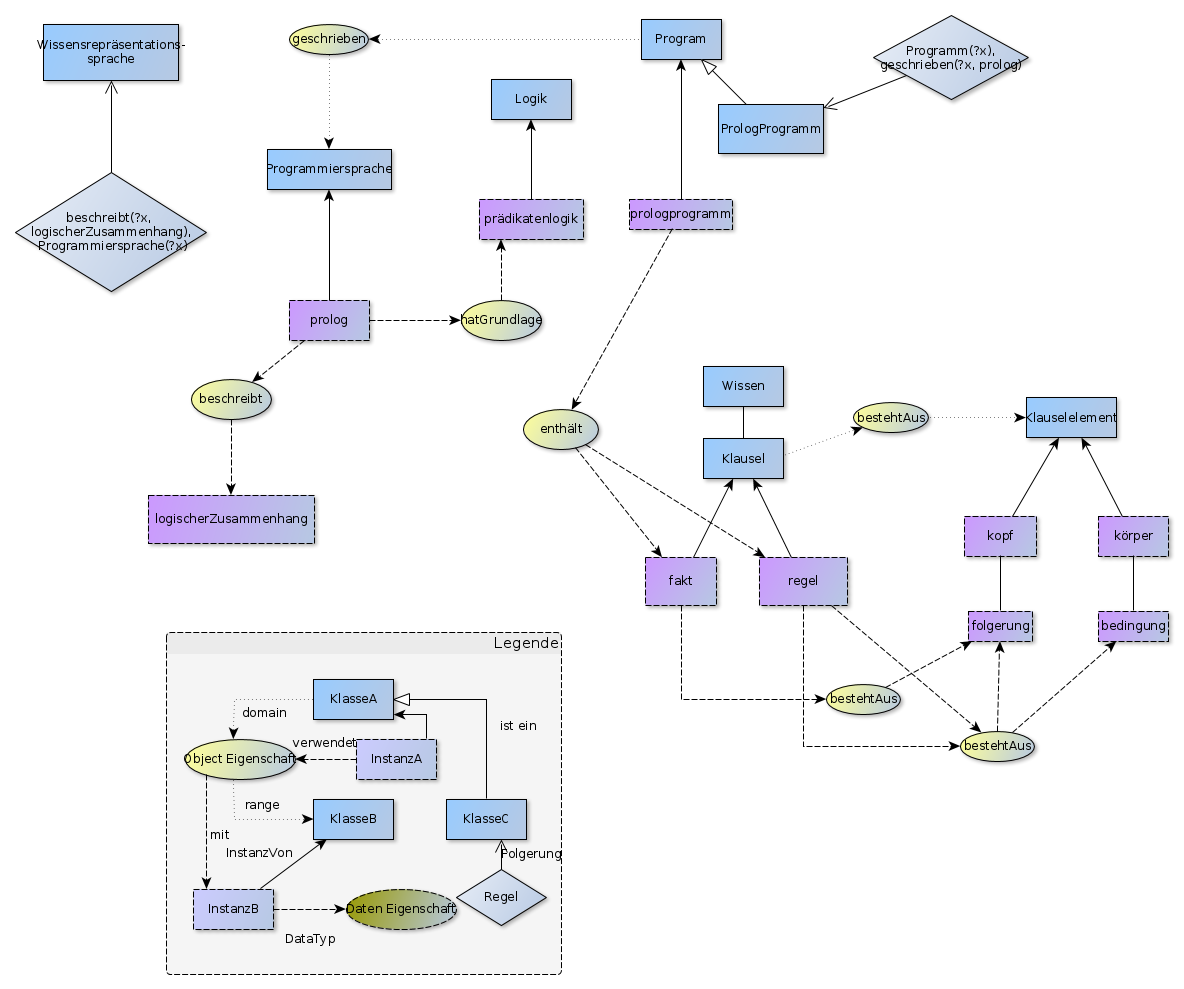
\includegraphics{bilder/prolog_netz.png}}}
\caption{Darstellung eines semantischen Netzes zur Abbildung von Prolog, mit Klassen, Individuen, Relationen und Regeln.\label{fig:prolog_netz}\protect\footnotemark}
\end{figure}
\footnotetext{Eigene Darstellung mittels yEd.}

Daher wurde eine andere Wissensdomäne --- die Planung von Reisen --- gewählt. Dies geht bereits eher in die Richtung von Expertensystemen, wofür semantische Netze am ehesten geeignet scheinen.

\subsection{Erstellung der Dokumentation zur Wissensmodellierung}
\label{subsec:dokumentation_wissensmodellierung}

\subsection{Erarbeitung der praktischen Grundlagen}
\label{subsec:praktische_grundlagen}

\subsection{Erstellung der abschliessenden Dokumentation}
\label{subsec:abschliessende_dokumentation}
